\documentclass[12pt]{article}
\usepackage{amsmath}
\usepackage[margin = 1in]{geometry}
\usepackage{graphicx}
\usepackage{booktabs}
\usepackage{hyperref}
\usepackage{cleveref}
\hypersetup{colorlinks = true, linkcolor = blue, citecolor=blue, urlcolor = blue}
\usepackage{natbib}
\usepackage{natbib}
\usepackage{float}
\usepackage{pdfpages}


\usepackage[colorlinks=true, citecolor=blue]{hyperref}



\title{UCSAS 2024 USOPC Data Challenge}
\author{Kathleen Houlihan\\
  Department of Statistics\\
  University of Connecticut
}

\begin{document}
\maketitle

\begin{abstract}
    For decades, gymnastics has been the most watched sport in the Summer Olympics and the United States 
    has been known for bringing gold medal-winning gymnasts to compete. In the 2020 
    Summer Olympics games in Tokyo, the United States female artistic gymnastics team took home 
    the gold medal in the Women's All Around, a bronze medal in the Women's Balance 
    Beam, a gold medal in the Women's Floor Exercise, a silver medal for the Women's
    Team, a bronze medal in the Women's Uneven Bars, and a silver medal in the Women's Vault. 
    Noting that the United States was the only country to have a team medal in all six women's artistic gymnastics 
    categories, the likely hood of the United States bringing female athletes that will medal in the 2024 
    Paris Olympics is very probable. However, in the 2020 Summer Olympic games in Tokyo, the United States 
    male artistic gymnastics team did not medal at all. For the purposes of this data challenge, I focused my 
    time on finding a statistical method that best isolates strong female gymnasts that would be prime candidates 
    for the 2024 olympics as the female USA team historically earns more medals than the male team. Later, I applied 
    my statistical method to the male team, which I anticipate will earn fewer medals than the female team, if any. 
    Noting that this data challenge can be interpreted in a number of ways, I designed my methods to maximize the 
    overall medal count while also placing greatest importance on the team all-around medal. In this paper, I will 
    identify which five female and male artistic gymnasts are best suited to be sent to the Paris 2024 
    Olympics on behalf of the United States in order to maximize the expected medal count. 

\end{abstract}


\section{Data}
\label{sec:data}

To predict which of the United States athletes are most likely to medal on the various apparatuses, 
I will be using the cleaned data that 
is provided in the UCSAS data challenge that includes data from major domestic and international 
gymnastic competitions from 2022 and 2023. I have opted against using the data from major domestic
and international gymnastic competions from 2017 to 2021 as time, injuries, 
and other factors can have a large impact on the success of a gymnast, so the greatest predictor
of the Olympic outcomes in 2024 will be the most recent data.
\\
For the purposes of my research design, when determining the most ideal feamle olympic candidates, 
I limited the data I utilized to only include female United States
gymnasts, presuming that the United States female gymnasts have a strong chance at earning medals in any category, 
based on the results of the 2020 Summer Olympics. When determining the most ideal American male candidates, 
I did inspect the data of non United States gymnasts in order to determine which medals the United States 
male team has the greatest chance of earning. 
Furthermore, I processed the data to remove any scores of zero based on the assumption that these may 
be indicative of missing scores and that instances of these scores are rare. I further justified my decision 
to eliminate scores of zero for the purposes of knowing the true mean scores of each athlete on each 
apparatus for each successful attempt. Additionally, for some athletes and competitions, I found that the vault
apparatus was listed as "VT," "VT1," and "VT2." This discrepancy is due to the fact that athletes are permitted
two attempts on the vault apparatus. In an effort to interpret the data as accurately as possible and avoid having 
multiple statistics for one athlete on the same apparatus, I corrected this discrepancy by merging "VT," "VT1," and 
"VT2" to all be reported as "VT." Also, the data source is flawed as it alternates between reporting athlete names
in upper or lower case letters. In order to correct this, I converted all last names to lower case for consistency 
purposes. Lastly, the data source is inconsistent in the manner that it reports the first names of athletes as certain
athletes are listed using only their first name at some competitions and are listed using their first and middle names 
under the "first name" category for other competitions. In order to resolve this discrepancy, I manually verified that 
any athletes listed under two names were the same person and I further verified that there were no United States  
athletes with the same last name so that all statistical computations could be completed through grouping by last 
name alone.

\section{Methods}
\label{sec:meth}

The most important task of the larger project involves determining which 5 athletes
should be brought to the 2024 Olympics in order to maximize success. For women, this means determining 
which five athletes stand the greatest chance of winning the gold medal for the women's individual all-around,
team all-around, Balance Beam, Floor Exercise, Uneven Bars, and Vault. 

In order to select the appropriate athletes, I first processed the data as described in Section~\ref{sec:data}.
Then, I calculated and examined the mean and standard deviations of each American female athlete's score 
on each apparatus. I also examined the number of observations for each athlete on each apparatus to familiarize 
myself with which athletes tend to compete at the most competitions and on which apparatuses. Then, I plotted 
the mean versus the standard deviation of the ten athletes with the highest mean scores on each apparatus. 
Using this visual, I created a parameter for each apparatus that uses both mean score and standard 
deviation to identify which athletes are best suited to be considered to compete on behalf of the United 
States on each apparatus. Using this parameter, I identified the "best" five athletes that compete on
each apparatus based on both their success, a high mean score, and their inconsistency, their standard deviation. 
In cases where there was only one observation, the standard deviation value is unavailable.
For the purposes of this research, it is reasonable to ignore any athletes who have only competed once on a particular apparatus.

Next, using only the athletes I identified as the "best" on each apparatus using the parameters, 
I calculated the sum of each athletes mean score for each apparatus and the sum of each athlete's standard 
deviation for each apparatus. Similarly to before, I plotted the mean score versus the standard deviation for 
these selected athletes. This plot is intended to represent
the United States' best candidates for earning a gold medal for the individual all-around component of the Olympics.

Then, using the sum of each selected athlete's mean score for each apparatus and the sum of each athlete's standard 
deviation for each apparatus which was previously calculated, I calculated the summed mean score and standard deviation sum 
of every combination of three athletes. Next, I plotted the summed mean score versus the standard deviation for the ten 
athlete combinations with the highest summed mean score. This plot is designed to identify the United States' best 
candidates for the all-around team finals.

Furthermore, using the sum of each selected athlete's mean score for each apparatus and the sum of each athlete's standard 
deviation for each apparatus which was previously calculated, I calculated the summed mean score and standard deviation sum 
of every combination of four athletes. Once again, I plotted the summed mean score versus the standard deviation for the ten 
athlete combinations with the highest summed mean score. This plot is designed to identify the United States' best 
candidates for the all-around team qualifying round.

Finally, in order to build a final team of five, I manually examined all of the data in an effort to include in 
the final team the best three candidates for the team all-around, the best candidate for the fourth qualifying position, 
the best two candidates for the individual all-around, and the two athletes that are superior on each apparatus.

For men, the overall statistical method I used to determine the team of five male gymnasts that should be sent 
to the 2024 Olympics was very similar, but varied when it came to determining the final fifth team member. After 
using the same method to determine the United States' best four male candidates for the team all-around qualification 
round, I calculated the mean score for every male gymnast on every apparatus in order to determine which apparatuses 
the male USA team had the greatest chance of earning medals on. From this data, there was only one additional male 
USA gymnast that ranked globally in the top ten for a particular apparatus based on mean score alone.

\section{Results}
\label{sec:res}

\begin{figure}
  \centering
  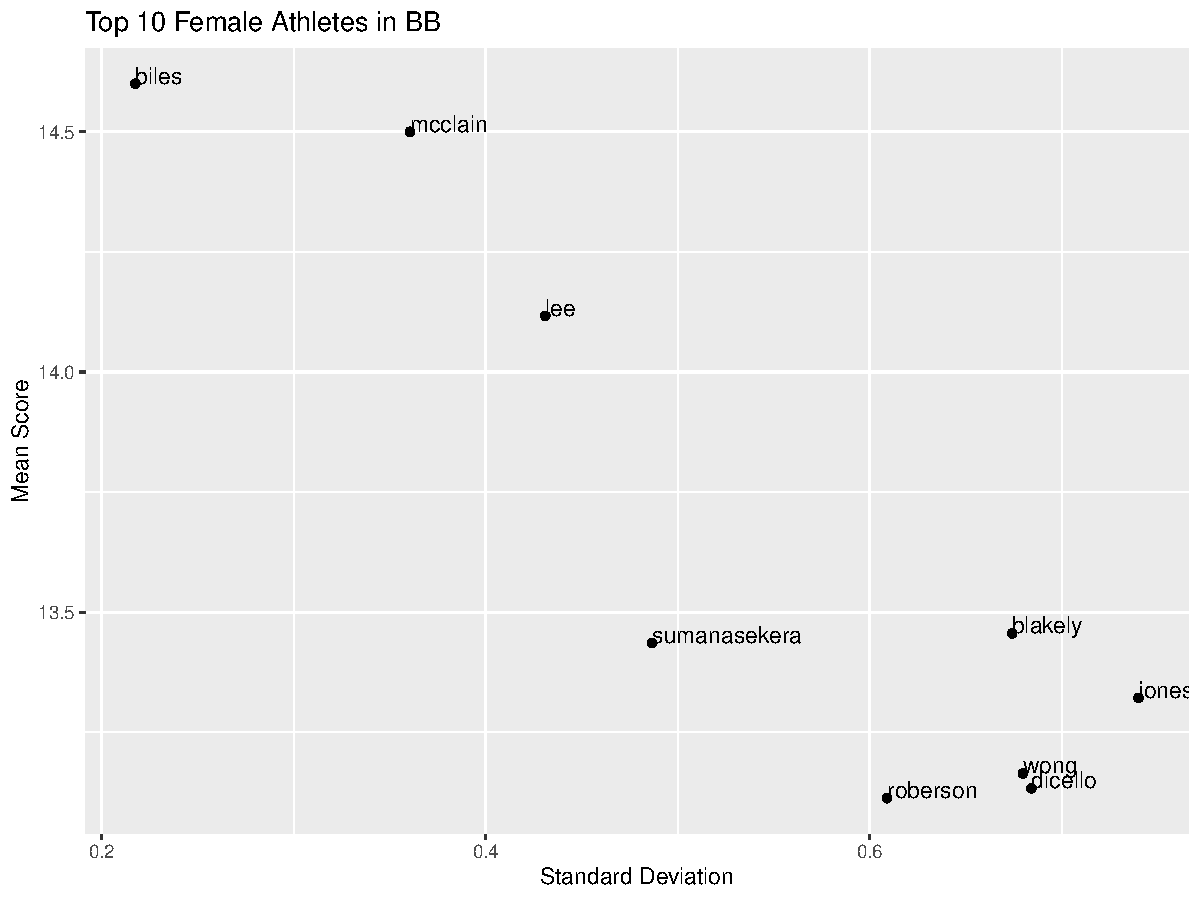
\includegraphics[scale=0.6]{FemaleAthletesBB.pdf}
  \caption{Top 10 Female Candidates for the Olympic Balance Beam Apparatus}
  \label{fig:BB}
\end{figure}

\begin{table}
  \caption{Top ten female balance beam candidates and their mean minus standard deviation parameter values}
  \label{tab:tableBBP}
\centering
\begin{tabular}[t]{lccllll}
 \toprule
Last Name & Mean minus Standard Deviation\\
\midrule
biles & 14.38228\\
\midrule
mcclain & 14.13944\\
\midrule
lee & 13.68558\\
\midrule
sumanasekera & 12.94901\\
\midrule
blakely & 12.78173\\
\midrule
jones & 12.58175\\
\midrule
roberson & 12.50378\\
\midrule
wong & 12.48469\\
\midrule
dicello & 12.44901\\
\midrule
frazier & NA\\
\bottomrule
\end{tabular}
\end{table}

Based on the plot of the top ten female athletes on the balance beam apparatus I selected the parameter of 
the score standard deviation subtracted from the mean score in order to identify the best suited five 
athletes. Based on the parameter, the five "best" female athletes on balance beam are Biles, Mcclain, 
Lee, Sumanasekera, and Blakely.


\begin{figure}
  \centering
  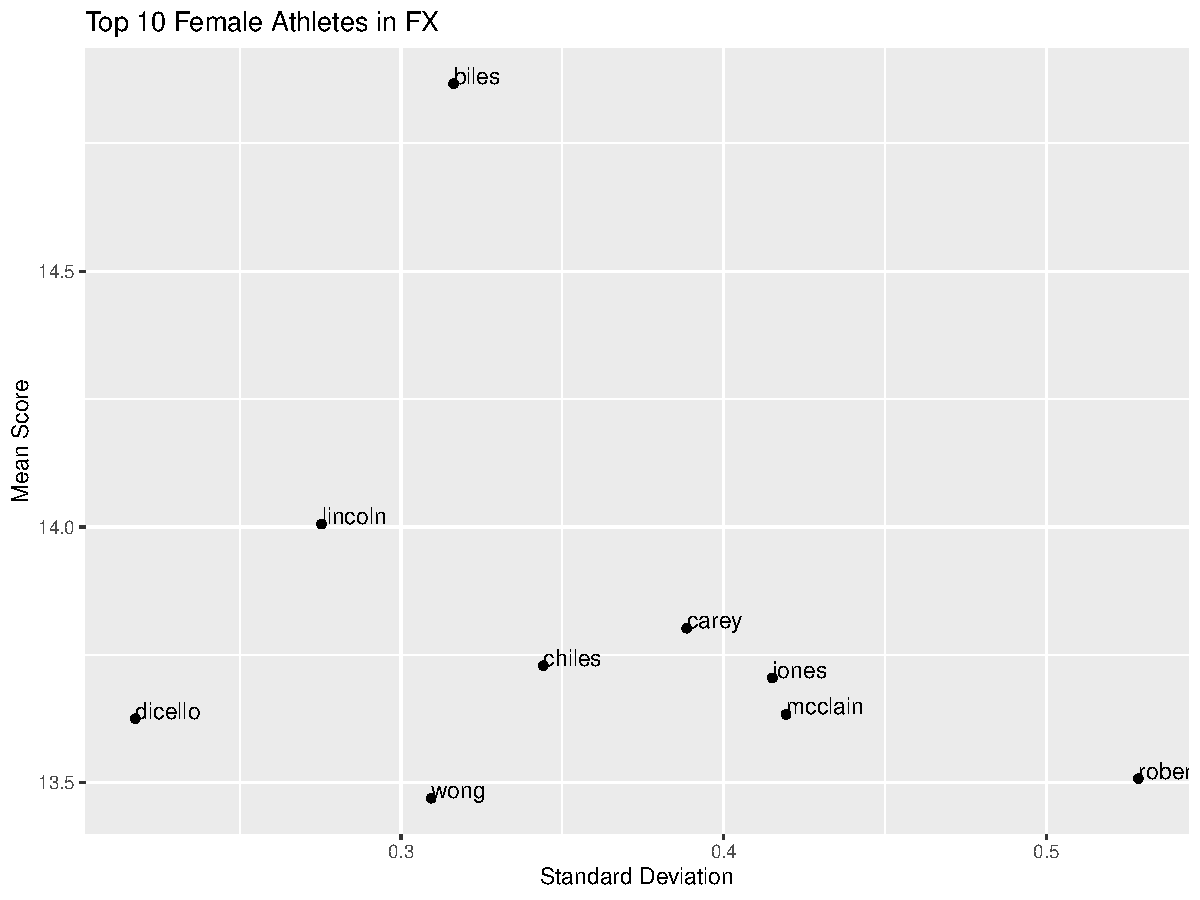
\includegraphics[scale=0.6]{FemaleAthletesFX.pdf}
  \caption{Top 10 Female Candidates for the Olympic Floor Exercise Apparatus}
  \label{fig:FX}
\end{figure}

\begin{table}
  \caption{Top ten female floor exercise candidates and their mean minus standard deviation parameter values}
  \label{tab:tableFXP}
\centering
\begin{tabular}[t]{lccllll}
 \toprule
Last Name & Mean minus Standard Deviation\\
\midrule
biles & 14.55017\\
\midrule
lincoln & 13.73014\\
\midrule
carey & 13.41335\\
\midrule
dicello & 13.40725\\
\midrule
chiles & 13.38463\\
\midrule
jones & 13.28955\\
\midrule
mcclain & 13.21401\\
\midrule
wong & 13.16001\\
\midrule
roberson & 12.97918\\
\midrule
frazier & NA\\
\bottomrule
\end{tabular}
\end{table}

Based on the plot of the top ten female athletes on the floor exercise apparatus I selected the parameter of 
the score standard deviation subtracted from the mean score in order to identify the best suited five 
athletes. Based on the parameter, the five "best" female athletes for floor exercise are Biles, Lincoln, Carey, 
Mcclain, Dicello, Chiles.

\begin{figure}
  \centering
  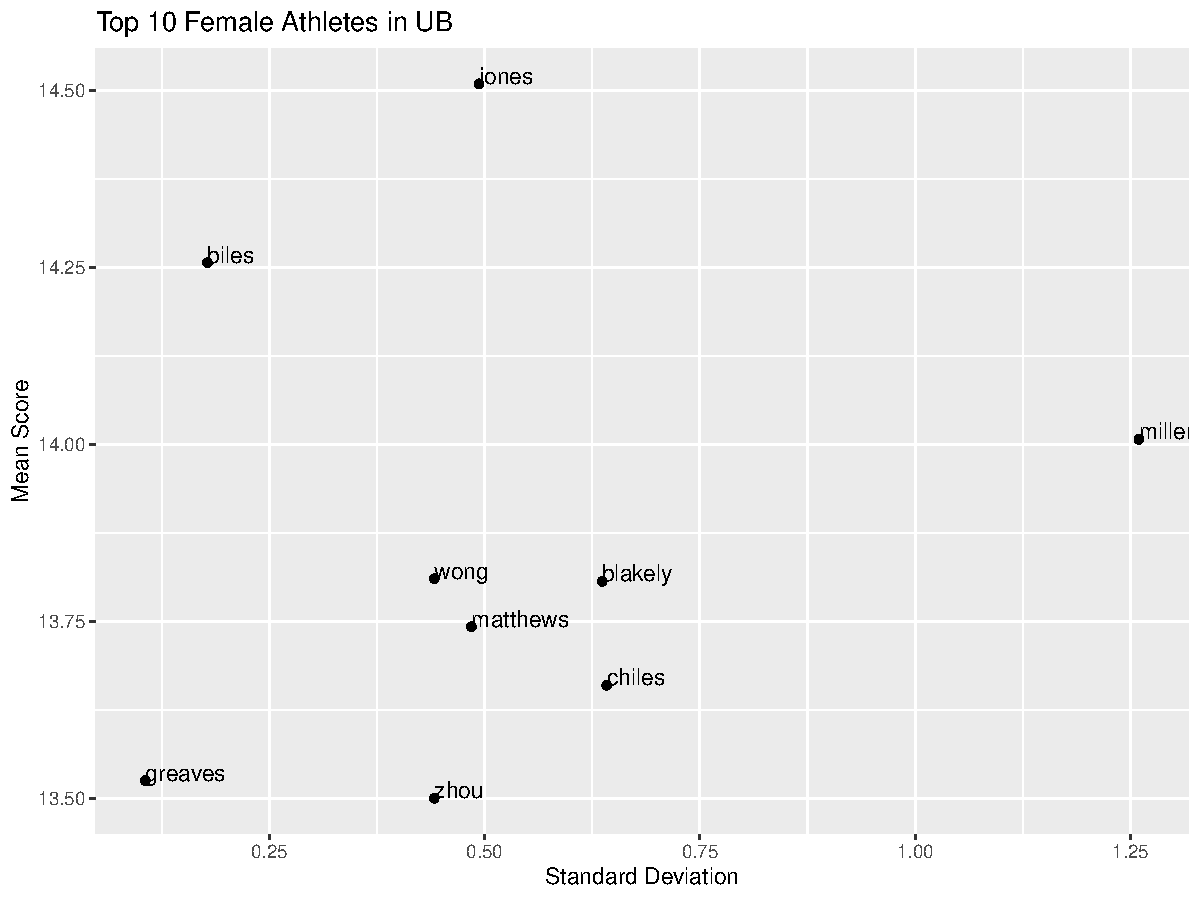
\includegraphics[scale=0.6]{FemaleAthletesUB.pdf}
  \caption{Top 10 Female Candidates for the Olympic Uneven Bar Apparatus}
  \label{fig:UB}
\end{figure}

\begin{table}
  \caption{Top 10 female uneven bars candidates and their mean minus half their standard deviation parameter values}
  \label{tab:tableUBP}
\centering
\begin{tabular}[t]{lccllll}
 \toprule
Last Name & Mean minus (0.5)Standard Deviation\\
\midrule
jones & 14.26300\\
\midrule
biles & 14.16786\\
\midrule
wong & 13.58939\\
\midrule
matthews & 13.50008\\
\midrule
blakely & 13.48821\\
\midrule
greaves & 13.47197\\
\midrule
miller & 13.37735\\
\midrule
chiles & 13.33873\\
\midrule
zhou & 13.27921\\
\midrule
walker & NA\\
\bottomrule
\end{tabular}
\end{table}

Based on the plot of the top ten female athletes on the uneven bars apparatus I selected the parameter of 
half of the score standard deviation subtracted from the mean score in order to identify the best suited five 
athletes. Based on the parameter, the five "best" female athletes for uneven bars are Jones, Biles, Wong, 
Matthews, and Blakely.

\begin{figure}
  \centering
  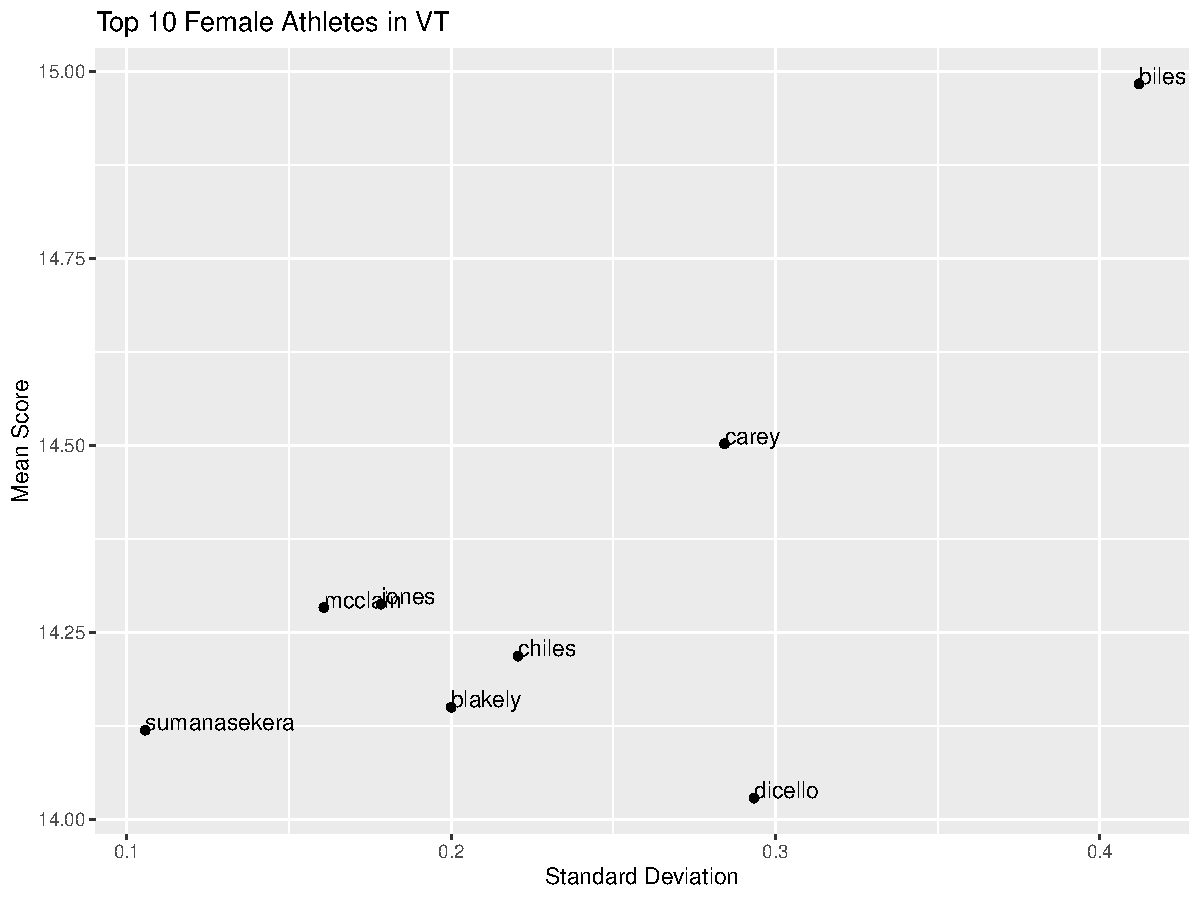
\includegraphics[scale=0.6]{FemaleAthletesVT.pdf}
  \caption{Top 10 Female Candidates for the Olympic Vault Apparatus}
  \label{fig:VT}
\end{figure}

\begin{table}
  \caption{Top ten female vault candidates and their mean minus half their standard deviation parameter values}
  \label{tab:tableVTP}
\centering
\begin{tabular}[t]{lccllll}
 \toprule
Last Name & Mean minus (0.5)Standard Deviation\\
\midrule
biles & 14.77708\\
\midrule
carey & 14.35999\\
\midrule
mcclain & 14.20297\\
\midrule
jones & 14.19854\\
\midrule
chiles & 14.10796\\
\midrule
sumanasekera & 14.06650\\
\midrule
blakely & 14.05000\\
\midrule
dicello & 13.88174\\
\midrule
richardson & NA\\
\midrule
torry & NA\\
\bottomrule
\end{tabular}
\end{table}

Based on the plot of the top ten athletes on the vault apparatus I selected the parameter of 
half of the score standard deviation subtracted from the mean score in order to identify the best suited five 
athletes. Based on the parameter, the five "best" female athletes on vault are Biles, Carey, Mcclain, Jones, 
and Chiles.

Ultimately, the list of athletes that ranked among the top five United States female athletes includes Biles, 
Mcclain, Lee, Sumanasekera, Blakely, Carey, Jones, Chiles, Wong, Matthews, Lincoln, and Dicello. However, Lee 
only has reported data for two out of four of the female apparatuses so she will not be considered with the other 
eleven athletes for individual or team all-around. Thus, the list of selected athletes that are involved in future 
computations includes Biles, Mcclain, Sumanasekera, Blakely, Carey, Jones, Chiles, Wong, Matthews, Lincoln, 
and Dicello.

\begin{figure}
  \centering
  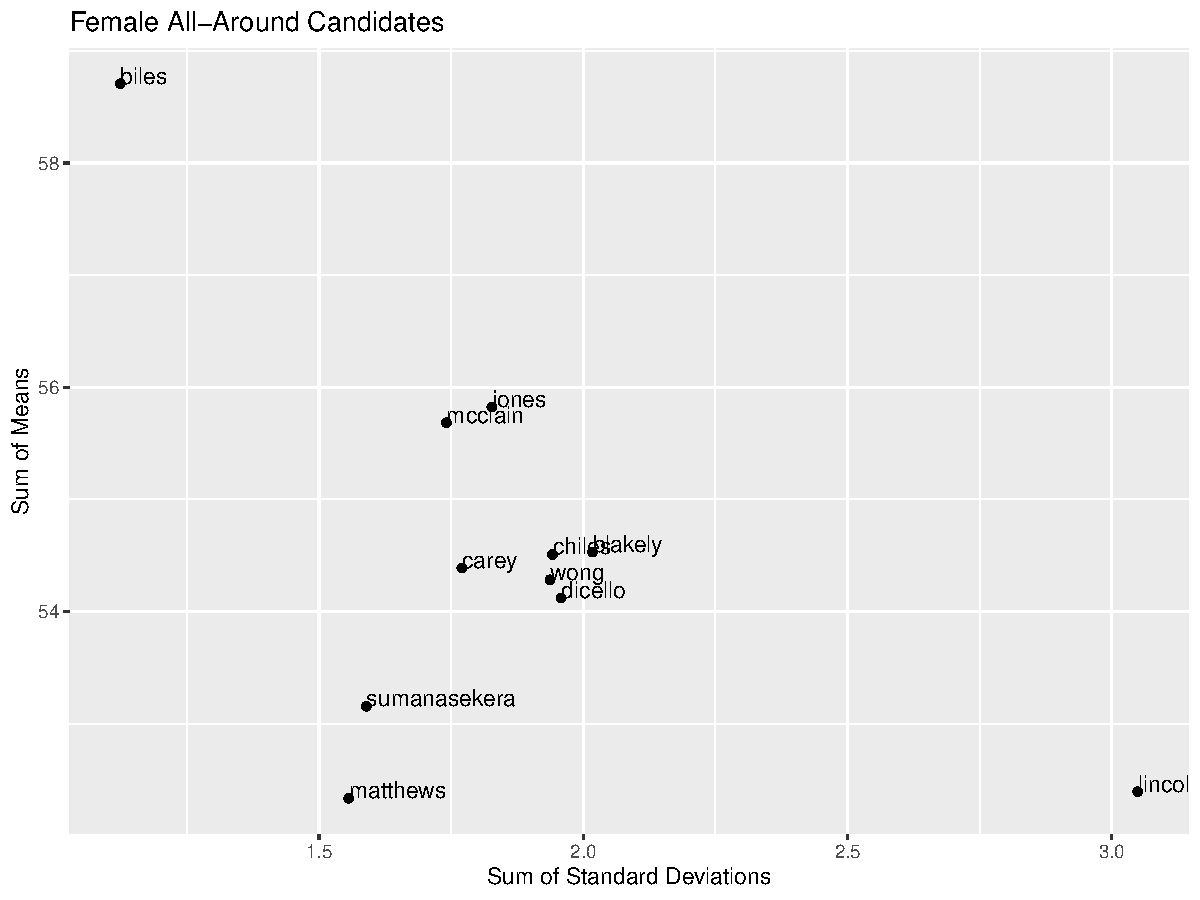
\includegraphics[scale=0.6]{FemaleAthletesAACandidates.pdf}
  \caption{The best candidates for the female individual all-around medal}
  \label{fig:IAA}
\end{figure}

\begin{table}
  \caption{Summed means and standard deviations for the selected female individual all-around candidates}
  \label{tab:tableIAA}
\centering
\begin{tabular}[t]{lccllll}
 \toprule
Last Name & Summed Means & Summed Standard Deviations\\
\midrule
biles & 58.70640 & 1.124194\\
\midrule
jones & 55.82380 & 1.826863\\
\midrule
mcclain & 55.68333 & 1.741128\\
\midrule
blakely & 54.52908 & 2.017384\\
\midrule
chiles & 54.50832 & 1.941718\\
\midrule
carey & 54.38711 & 1.770006\\
\midrule
wong & 54.28354 & 1.936921\\
\midrule
dicello & 54.11984 & 1.958245\\
\midrule
sumanasekera & 53.15505 & 1.589704\\
\midrule
lincoln & 52.39283 & 3.048907\\
\midrule
matthews & 52.33400 & 1.556188\\
\bottomrule
\end{tabular}
\end{table}

Figure~\ref{fig:IAA} and table~\ref{tab:tableIAA} display the summed mean score and standard deviation 
for each of the eleven selected female all-around candidates.

\begin{figure}
  \centering
  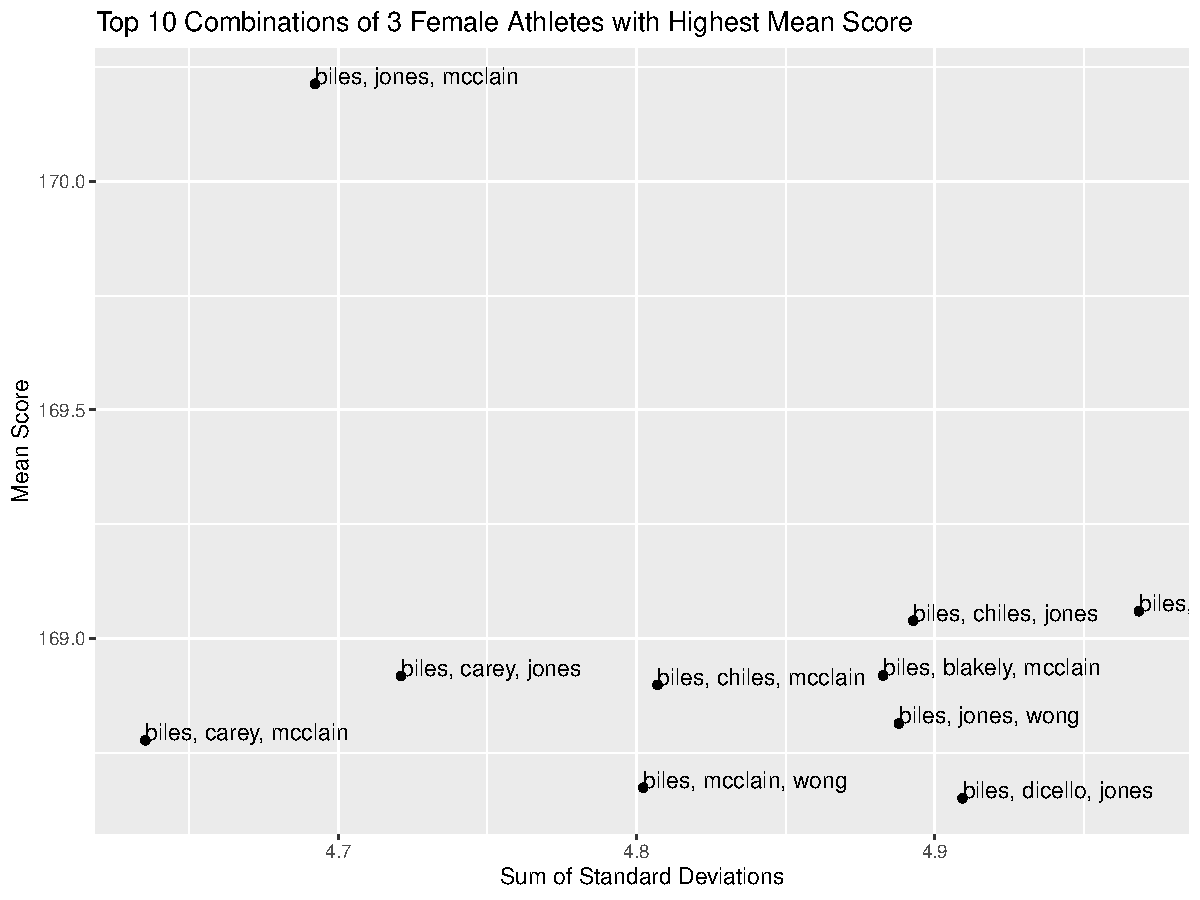
\includegraphics[scale=0.6]{FemaleAthletesAA3.pdf}
  \caption{Top 10 combinations of three female candidates for the team all-around medal}
  \label{fig:AA3}
\end{figure}

\begin{table}
  \caption{The five combinations of three United States female athletes with the highest combined mean scores}
  \label{tab:tableAA3}
\centering
\begin{tabular}[t]{lccllll}
 \toprule
Combination & Combined Score & Standard Deviation Sum\\
\midrule
biles, jones, mcclain & 170.2135 & 4.692185\\
\midrule
biles, blakely, jones & 169.0593 & 4.968440\\
\midrule
biles, chiles, jones & 169.0385 & 4.892774\\
\midrule
biles, blakely, mcclain & 168.9188 & 4.882706\\
\midrule
biles, carey, jones
& 168.9173 & 4.721063
\\
\bottomrule
\end{tabular}
\end{table} 

Figure~\ref{fig:AA3} and table~\ref{tab:tableAA3} display the summed mean score and standard deviation 
for the top combinations of three of the eleven selected female all-around candidates.

\begin{figure}
  \centering
  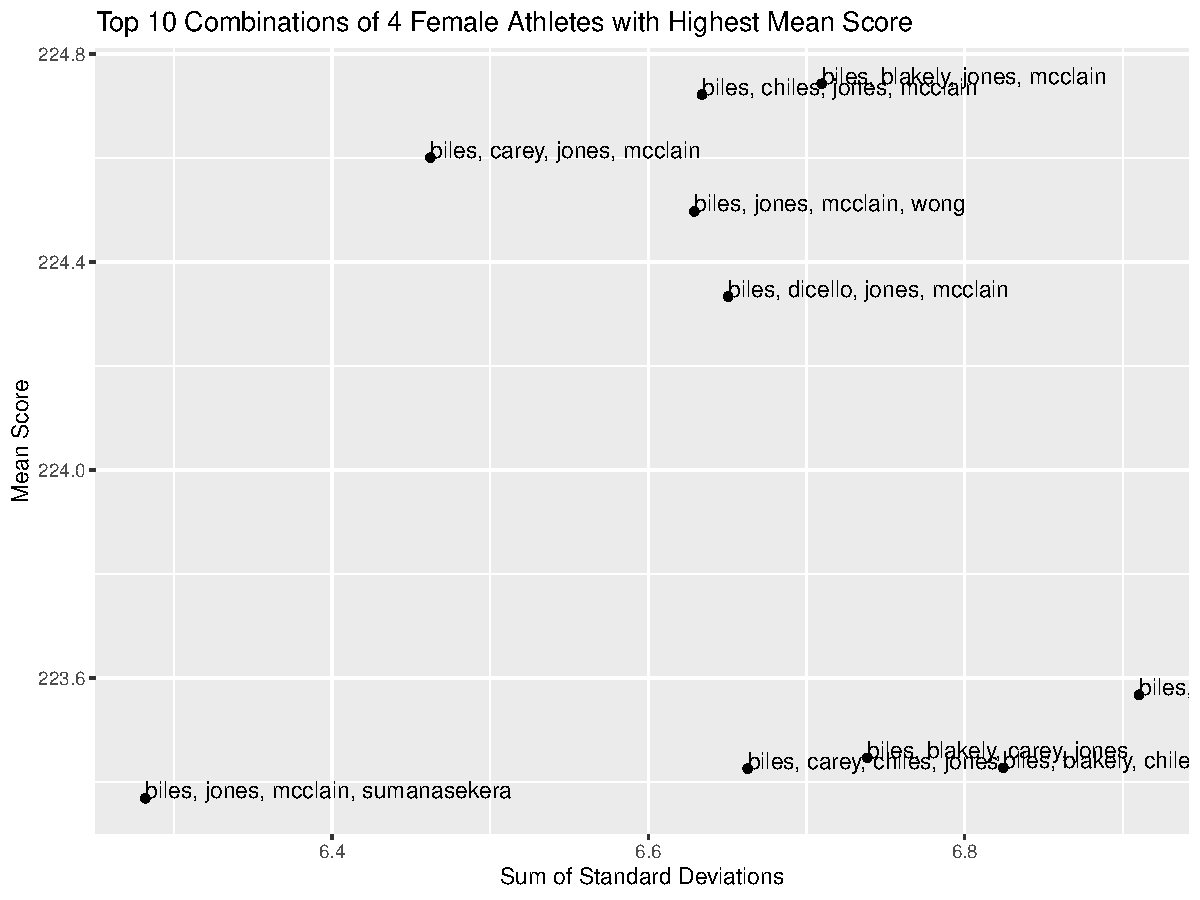
\includegraphics[scale=0.6]{FemaleAthletesAA4.pdf}
  \caption{Top 10 combinations of four female candidates for the team all-around medal}
  \label{fig:AA4}
\end{figure}

\begin{table}
  \caption{The five combinations of four United States female athletes with the highest combined mean scores}
  \label{tab:tableAA4}
\centering
\begin{tabular}[t]{lccllll}
 \toprule
Combination & Combined Score & Standard Deviation Sum\\
\midrule
biles, blakely, jones, mcclain & 224.7426 & 6.709569\\
\midrule
biles, chiles, jones, mcclain & 224.7218 & 6.633903\\
\midrule
biles, carey, jones, mcclain & 224.6006 & 6.462191\\
\midrule
biles, jones, mcclain, wong & 224.4971 & 6.629105\\
\midrule
biles, dicello, jones, mcclain & 224.3334 & 6.650430\\
\bottomrule
\end{tabular}
\end{table} 

Figure~\ref{fig:AA4} and table~\ref{tab:tableAA4} display the summed mean score and standard deviation 
for the top combinations of four of the eleven selected all-around candidates.

\begin{figure}
    \centering
    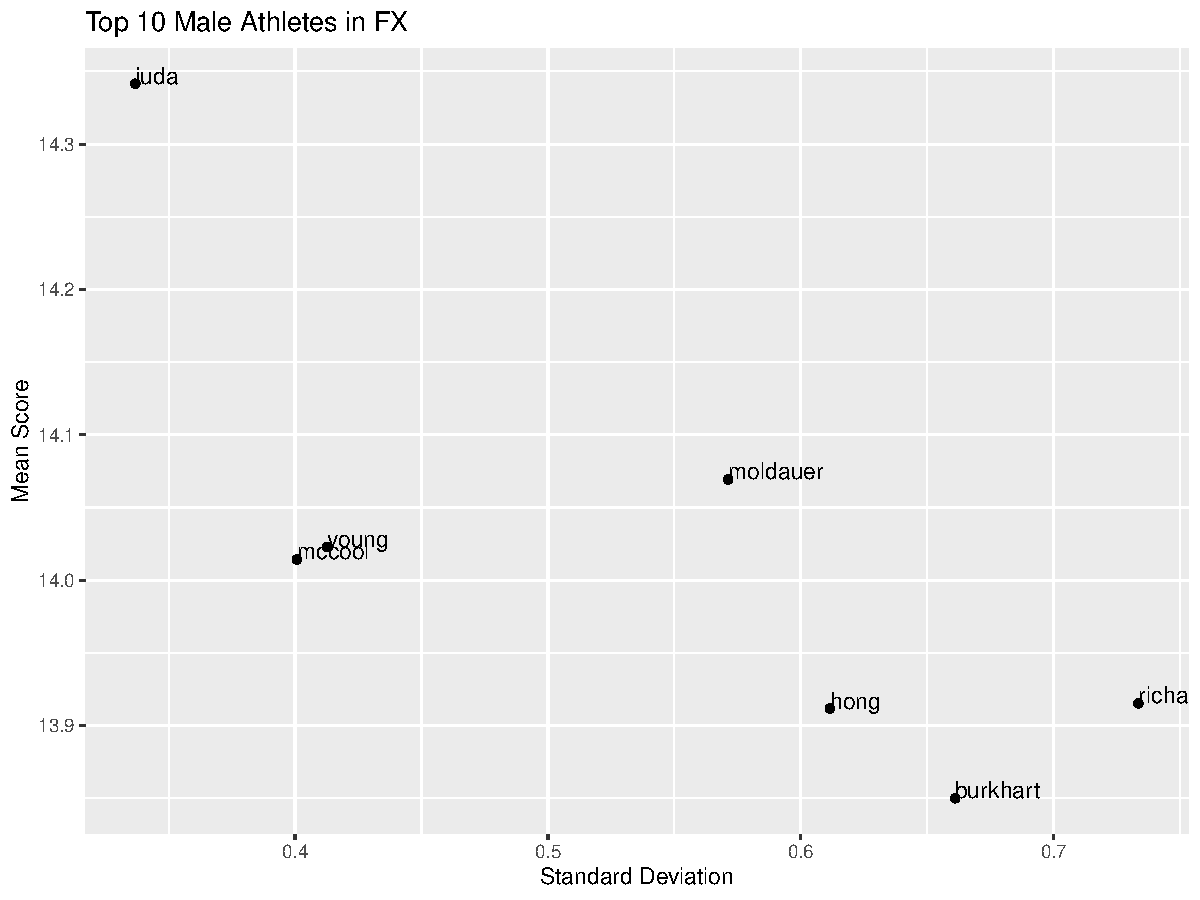
\includegraphics[scale=0.6]{MaleAthletesFX.pdf}
    \caption{Top 10 Male Candidates for the Olympic Floor Exercise Apparatus}
    \label{fig:FXM}
  \end{figure}

  Based on the plot of the top ten male athletes on the floor exercise apparatus I selected the parameter of 
  the score standard deviation subtracted from the mean score in order to identify the best suited five 
  athletes. Based on the parameter, the five "best" male athletes on floor exercise are Juda, Mccool, Young, Moldauer, 
  and Hong.

\begin{figure}
    \centering
    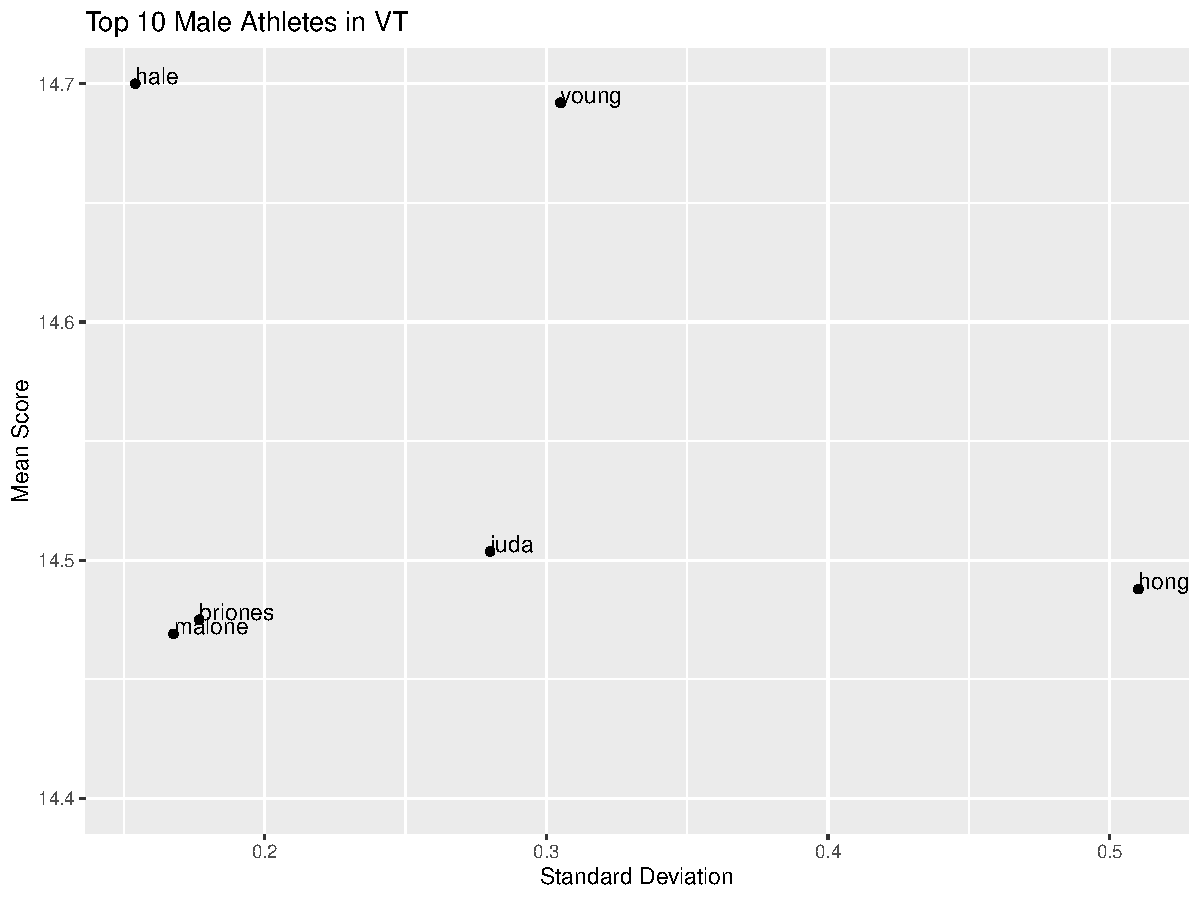
\includegraphics[scale=0.6]{MaleAthletesVT.pdf}
    \caption{Top 10 Male Candidates for the Olympic Vault Apparatus}
    \label{fig:VTM}
  \end{figure}

  Based on the plot of the top ten male athletes on the vault apparatus I selected the parameter of 
  the score standard deviation subtracted from the mean score in order to identify the best suited five 
  athletes. Based on the parameter, the five "best" male athletes on vault are Hale, Young, Malone, Briones, and 
  Juda.

\begin{figure}
    \centering
    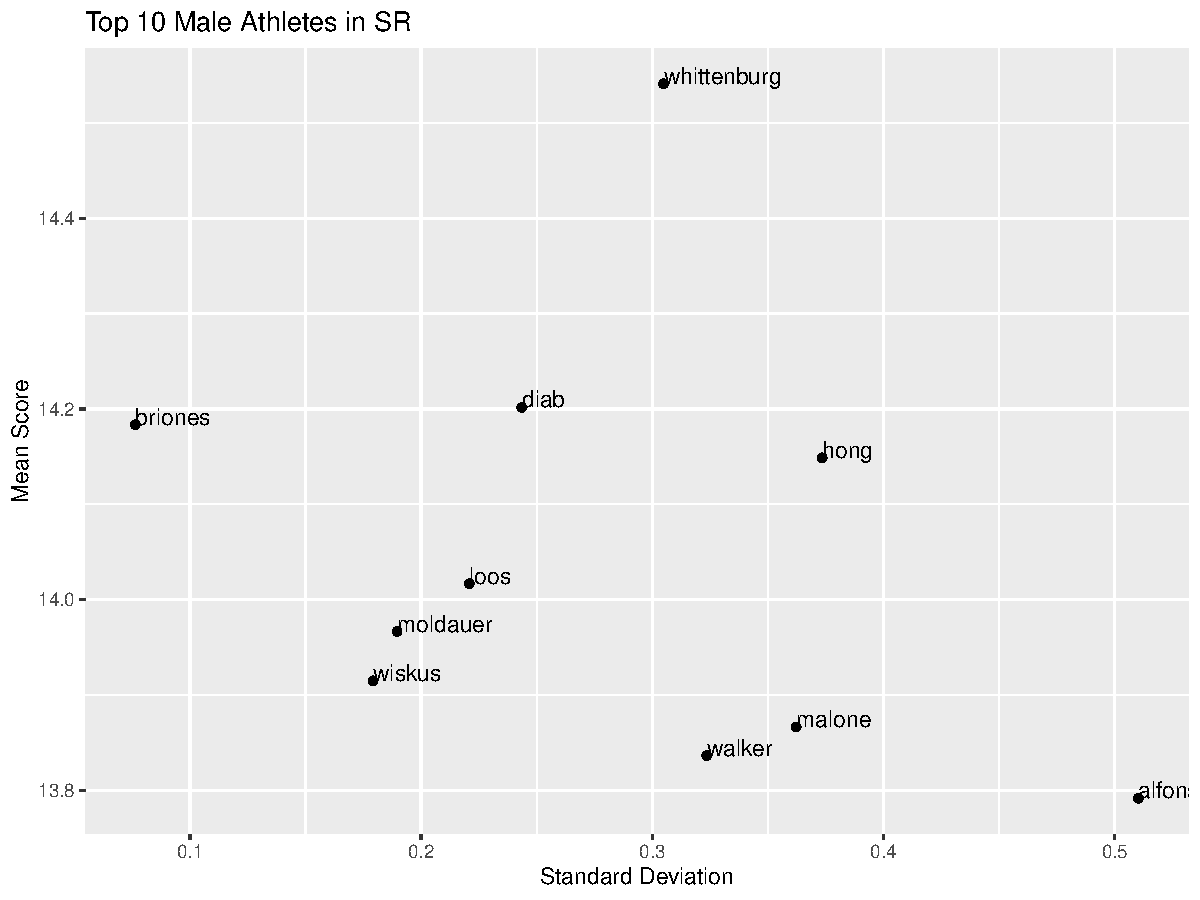
\includegraphics[scale=0.6]{MaleAthletesSR.pdf}
    \caption{Top 10 Male Candidates for the Olympic Still Rings Apparatus}
    \label{fig:SRM}
  \end{figure}

  Based on the plot of the top ten male athletes on the still rings apparatus I selected the parameter of 
  half of the score standard deviation subtracted from the mean score in order to identify the best suited five 
  athletes. Based on the parameter, the five "best" male athletes on still rings are Whittenburg, Briones, Diab, 
  Hong, and Loos.

\begin{figure}
    \centering
    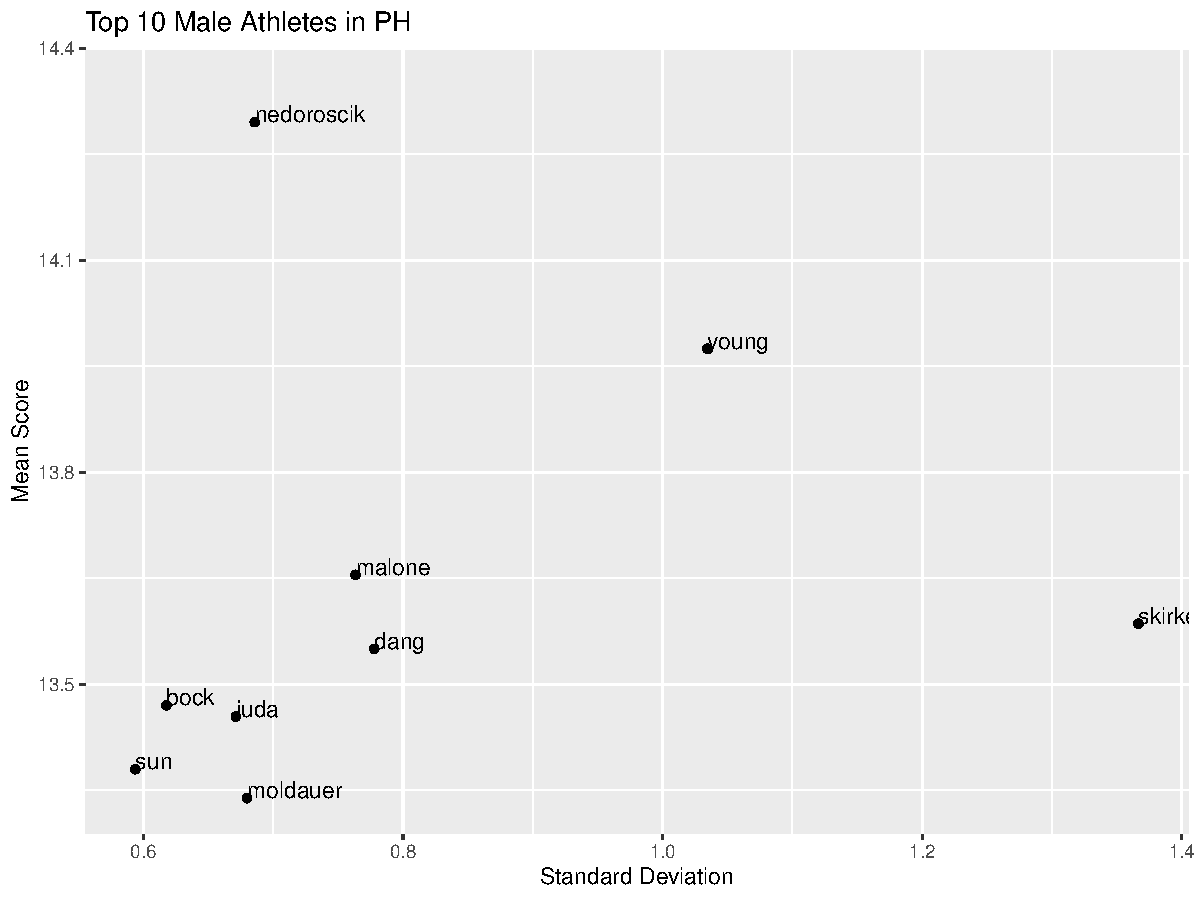
\includegraphics[scale=0.6]{MaleAthletesPH.pdf}
    \caption{Top 10 Male Candidates for the Olympic Pommel Horse Apparatus}
    \label{fig:PHM}
  \end{figure}

  Based on the plot of the top ten male athletes on the pommel horse apparatus I selected the parameter of 
  half of the score standard deviation subtracted from the mean score in order to identify the best suited five 
  athletes. Based on the parameter, the five "best" male athletes on pommel horse are Nedoroscik, Young, Malone, 
  Dang, and Bock.

\begin{figure}
    \centering
    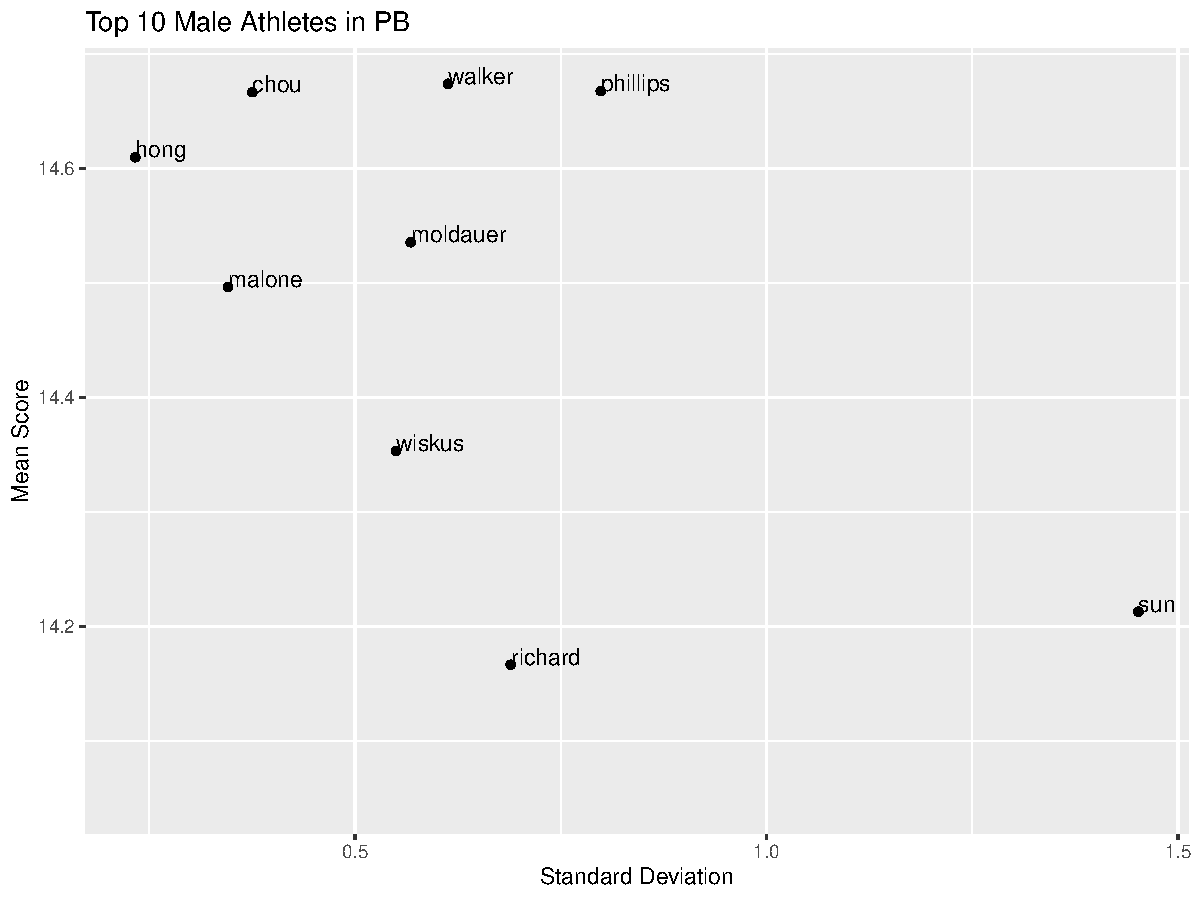
\includegraphics[scale=0.6]{MaleAthletesPB.pdf}
    \caption{Top 10 Male Candidates for the Olympic Parallel Bars Apparatus}
    \label{fig:PBM}
  \end{figure}

  Based on the plot of the top ten male athletes on the parallel bars apparatus I selected the parameter of 
  half of the score standard deviation subtracted from the mean score in order to identify the best suited five 
  athletes. Based on the parameter, the five "best" male athletes on parallel bars are Hong, Chou, Walker, Malone, 
  and Phillips.

\begin{figure}
    \centering
    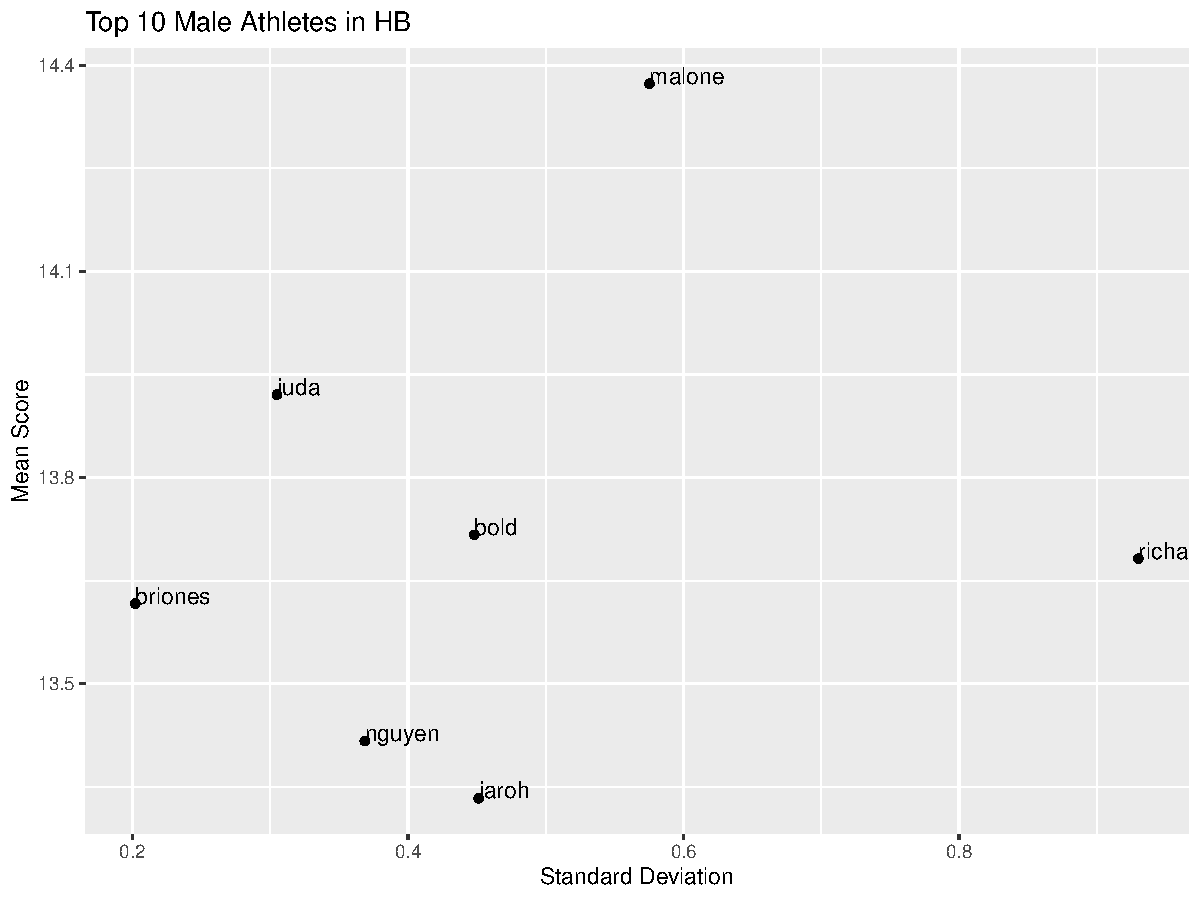
\includegraphics[scale=0.6]{MaleAthletesHB.pdf}
    \caption{Top 10 Male Candidates for the Olympic High Bar Apparatus}
    \label{fig:HBM}
  \end{figure}

  Based on the plot of the top ten male athletes on the high bar apparatus I selected the parameter of 
  half of the score standard deviation subtracted from the mean score in order to identify the best suited five 
  athletes. Based on the parameter, the five "best" male athletes on high bar are Malone, Juda, Briones, Bold, and 
  Nguyen.

  Ultimately, the list of athletes that ranked among the top five United States male athletes 19 distinct 
  names. However, nine of these athletes have not competed on all six apparatuses, so they will not be considered 
  with the other ten athletes for individual or team all-around. Thus, the list of selected athletes that 
  are involved in future computations includes Juda, Young, Moldauer, Hong, Hale, Malone, Whittenburg, Loos, 
  Bock, and Walker.

\begin{figure}
    \centering
    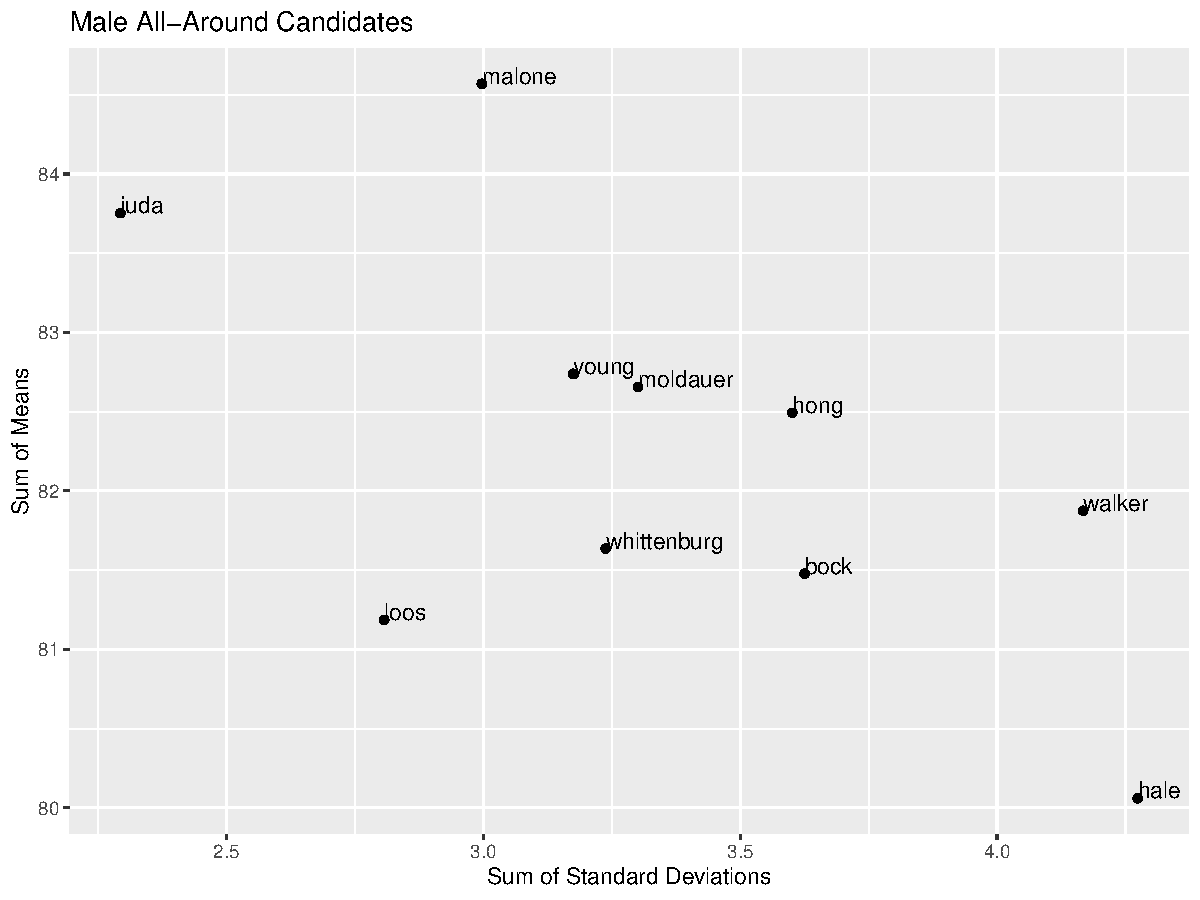
\includegraphics[scale=0.6]{MaleAthletesAACandidates.pdf}
    \caption{The best candidates for the male individual all-around medal}
    \label{fig:IAAM}
  \end{figure}

  Figure~\ref{fig:IAAM} displays the summed mean score and standard deviation 
  for each of the ten selected male all-around candidates.

\begin{figure}
    \centering
    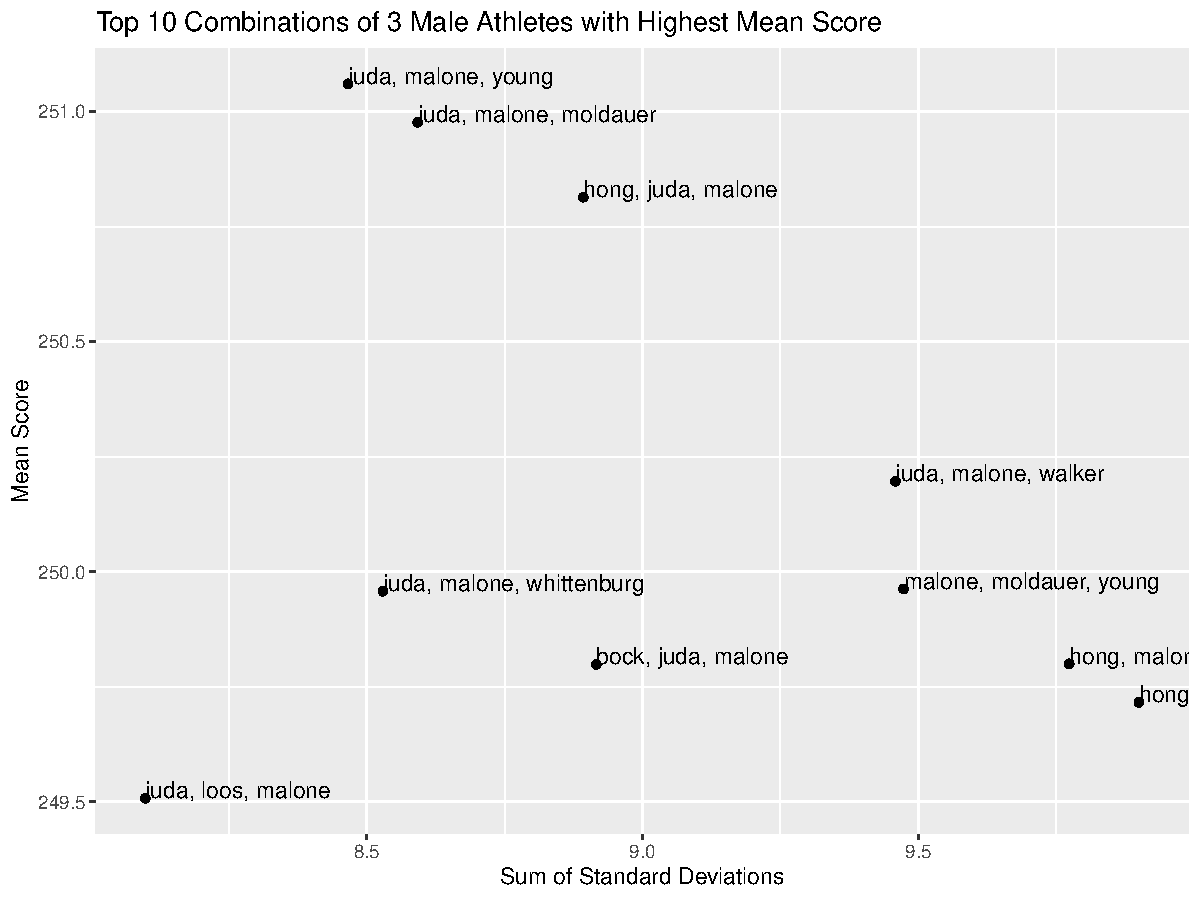
\includegraphics[scale=0.6]{MaleAthletesAA3.pdf}
    \caption{Top 10 combinations of three male candidates for the team all-around medal}
    \label{fig:MAA3}
  \end{figure}

  Figure~\ref{fig:MAA3} displays the summed mean score and standard deviation 
  for the top combinations of three of the ten selected male all-around candidates.
  
  \begin{figure}
    \centering
    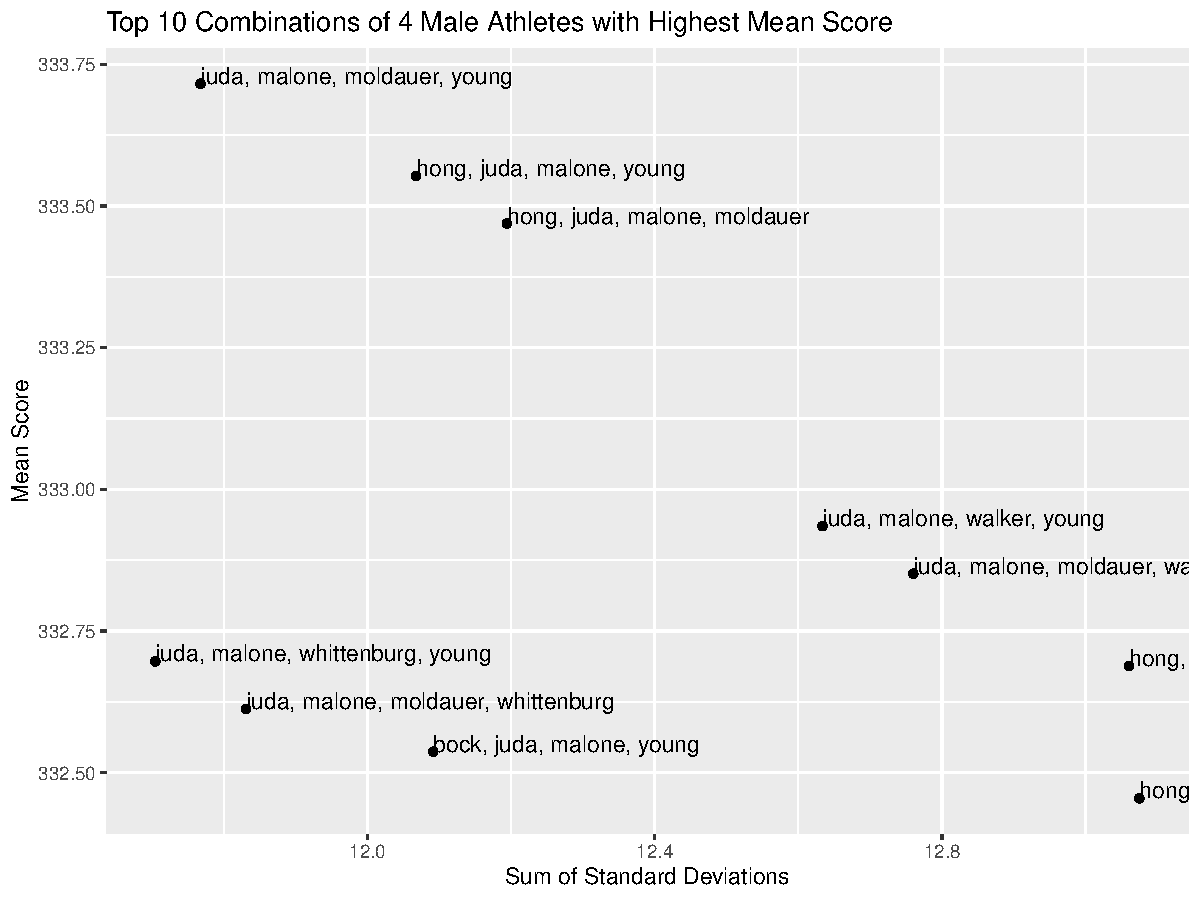
\includegraphics[scale=0.6]{MaleAthletesAA4.pdf}
    \caption{Top 10 combinations of four male candidates for the team all-around medal}
    \label{fig:MAA4}
  \end{figure}

  Figure~\ref{fig:MAA4} displays the summed mean score and standard deviation 
  for the top combinations of four of the ten selected male all-around candidates.

\section{Discussion}
\label{sec:dis}

In my preliminary steps, I calculated the mean and standard deviation for every female athlete on each 
apparatus they were reported to have competed on. From these calculations, I decided to cut out most athletes 
by only inspecting athletes that ranked in the top ten by mean score alone for each apparatus. This was a 
reasonable elimination of data as the score values among the top ten candidates varied enough, often by over a 
full point, to justify that athletes that never ranked in the top ten for a particular apparatus are not 
competitive enough to medal at the Olympics.

I later developed a parameter for each apparatus to further reduce the list of athletes to only include athletes 
that rank in the top five for each apparatus. However, I designed the parameters to be dependent on the score 
standard deviation in addition to the mean score. The intent of the paramter is to create a frontier that selects 
athletes that have high mean scores and low standard deviations in order to select athletes that are the most 
successful and consistent. Ultimately, for each apparatus I selcted the five athletes with highest parameter value.

For the blanace beam apparatus, I selected the parameter: mean score minus standard deviation. This parameter 
is very reasonable as it selects athletes with high means and low standard deviations first (Biles then Mcclain 
then Lee) and selects athletes with lower standard deviations when means are similar (Sumanasekera then Blakely).

For the floor exercise apparatus, I selected the parameter: mean score minus standard deviation. This parameter 
is reasonable as well as it selects athletes with high means and low standard deviations first (Biles then Lincoln) 
and selects athletes with lower standard deviations when means are similar (Carey, Dicello, and Chiles). Note, the 
order in which Carey, Dicello, and Chiles "should" be selected is debatable, but it is most important that the 
parameter selected these athletes as opposed to athletes that have similar mean scores but higher standard deviations 
(Jones and Mcclain) or low standard deviations and low low mean scores (Wong).

For the uneven bars apparatus, I selected the parameter: mean score minus half of the standard deviation. 
This parameter is reasonable as well as it selects athletes with extremely high means first (Jones then Biles) and selects 
athletes with lower standard deviations when means are similar (Wong then Matthews then Blakely). 

For the vault apparatus, I selected the parameter: mean score minus half of the standard deviation. 
This parameter is reasonable as well as it selects athletes with extremely high means first (Biles then Carey) and selects 
athletes with lower standard deviations when means are similar (Mcclain then Jones then Chiles). 

Then, I used these candidates in order to determine who is best suited to compete in the all-around events. 
First, I calculted the summed mean score and summed standard deviation for each selected athlete. Looking at the data 
values and plot of these individual all-around candidates, it is very clear that Biles is strong candidate to 
compete for the individual all-around medal. However, it is not clear whether Jones or Mcclain is better suited 
to be the second United States individual all-around candidate.

Then, I used the summed mean score and summed standard deviation for each selected athlete to calculate the 
summed mean score and summed standard deviation for every combination of 
three and four of these selected athletes. Looking at the data values and plot of the combinations of three athletes, 
it is clear that Biles, Jones, and Mcclain are by far the best suited trio to compete for the team all-around medal. 
Additionally, since this data suggests that both Mcclain and Jones should compete in the qualifying round, there 
is no need to select one over the other for the second individual all-around candidate spot as they would both get 
the opportunity to qualify, and their scores at the Olympics will determine which athlete, if either, will qualify 
to attend the individual all-around finals. 

Looking at the data values and plot of the combinations of four athletes, it is not clear whether Chiles, Carey, or 
Blakely is best suited to be the fourth team all-around candidate as their means and standard deviations are very 
similar. However, looking at the individual apparatus events provides justification for who to ultimately select. 
Knowing that two athletes per country can compete for an apparatus medal, it is strategic to try to compose the 
team of the best two United States athletes for each apparatus. Based on the computations and plots, the superior two 
athletes on balance beam are Biles and Mcclain, the superior two athletes on floor exercise are Biles and Lincoln, 
the superior two athletes on uneven bars are Jones and Biles, and the superior two athletes on vault are Biles 
and Carey. Since Lincoln was not among our top candidates for an all-around medal, it would be logical to select her 
as the fifth United States Olympic team member who does not compete in the all-around qualifying round. Additionally, 
since Carey is one of the candidates being considering for the all-around qualifying round and she is one of our superior 
athletes on vault, it is reasonable to also select her to be the final member of the Olympic team. Although, the 
summed combination that included Carey has the lowest mean in comparison to the combinations including Chiles or 
Blakely, the selection of Carey can be further justified by the facts that the summed mean score difference is 
within one point the combination including Carey has the lowest summed standard deviation.

Ultimately, in order to maximize the the number of medals the Unites States female team wins, I would comprise the 
team of the athletes Biles, Jones, Mcclain, Lincoln, and Carey.

Similarly, I used the same method to determine the "best" male all-around candidates as I did for females. From 
Figure~\ref{fig:IAAM} I determined that Juda and Malone are the best male Individual all-around candidates. From 
Figure~\ref{fig:MAA3} I determined that Juda, Malone, and Young are the best male team all-around finalists 
candidates. Additionally, from Figure~\ref{fig:MAA4} I determined that Moldauer is the best candidate to also compete 
with Juda, Malone, and Young in the all-around qualifying round. Comparatively, determining the "best" fifth Olympic 
teammate is challenging as there are several apparatuses where our "best" competitor is not among the four 
previously selected teammates. However, through examining the the mean score for every male gymnast on every apparatus 
we can see that many of our "best" candidates are still ranked very poorly globally, and therefore would not have a 
strong liklihood of medalling at the olympics. Among all of the male USA athletes that are not yet selected, the only 
athlete that has a relatively decent chance of medaling is Hale, who ranks 6th globally for the Vault apparatus.

Ultimately, in order to maximize the the number of medals the Unites States male team wins, I would comprise the 
team of the athletes Juda, Malone, Young, Moldauer, and Hale.


\end{document}